\section{Einleitung}
\label{s:intro}

Hier kommt die Einleitung.


%%%%%%%%%%%%%%%%%%%%%%%%%%%%%%%%%%%%%%%%%%%%%%%%%%%%%%%%%%%%%%
\subsection{Ein Abschnitt der Einleitung}
\label{ss:intro:abc}

Einen Überblick findet man z.\,B.\ in \cite{Auer00:HTF}.

\begin{figure}[t]
\centering

\begin{subfigure}{0.45\linewidth}
\centering
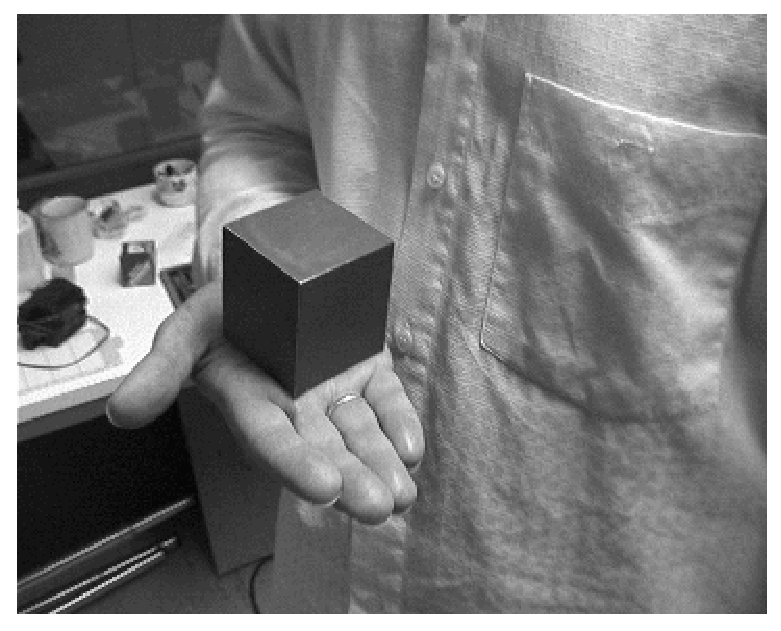
\includegraphics[width=\linewidth]{\figdir/handorig}
\caption{Originalbild}
\label{FIG:arexorig}
\end{subfigure}
%
\begin{subfigure}{0.45\linewidth}
\centering
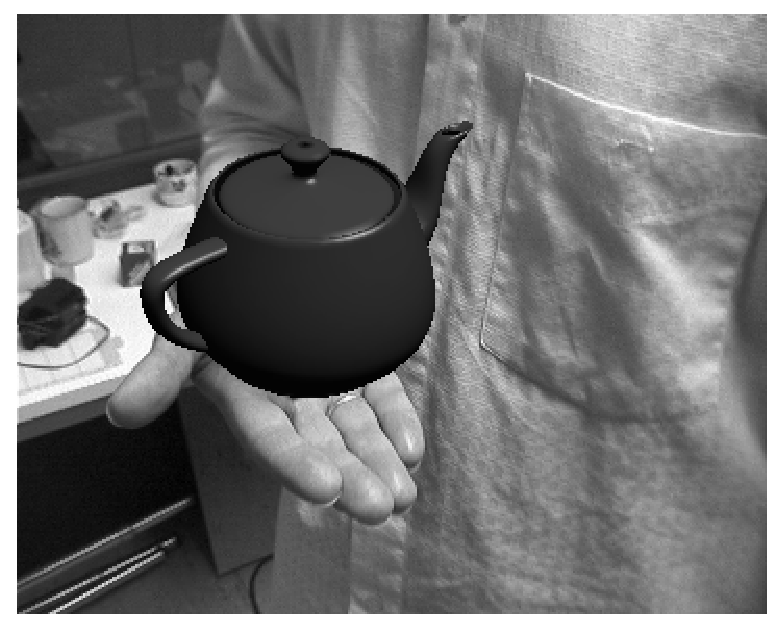
\includegraphics[width=\linewidth]{\figdir/handaug}
\caption{erweitertes Bild}
\label{FIG:arexaugm}
\end{subfigure}
%
\caption[AR Beispiel]
{Beispiel eines Augmented Reality Systems: es folgt eine Beschreibung (Bilder aus \cite{Schmidt01:PAO})}
\label{FIG:arex}
\end{figure}

Ein Beispiel wird in Abb.\ \ref{FIG:arex} gezeigt.
Das verwendete Objekt ist in Abb.\ \ref{FIG:arexorig} dargestellt, das Ergebnis in Abb.\ \ref{FIG:arexaugm}.

Eine Formel
\begin{equation}
\label{eq:cvp:test}
f(x) = \frac{1}{3} x + 5, \quad x \in \real.
\end{equation}

Und noch eine:
\begin{equation}
\label{eq:cvp:matvec}
\bm{M}  = \bm{Ax} \pi, \quad \bm{A} \in \real^{2 \times 2}, \bm{x} \in \real^2.
\end{equation}

Tabelle \ref{t:CodebookOverview} gibt einen Überblick über XYZ.

\begin{table}[t]
\centering\small
%
% generated by TexTableGenerator.pl ((c) Florian Vogt)
% from file: /home/Jochen/data/dissdata/results/CodebookOverview.log
%
\begin{tabular}{l|ccc|cc}
\hline
\hline
                  \textbf{Sequence} &          ARTS &           wman &         stcams &         ARTVZ &        ARTSUZ \\ 
                 \textbf{\# Frames} &             190 &              40 &             400 &             270 &             190 \\ 
     \textbf{\# relative movements} &           17955 &             780 &           79800 &           36315 &           17955 \\ 
\textbf{\# movements after pre-sel.} &           14336 &             623 &           37915 &           21788 &           14343 \\ 
       \textbf{min.\ angle in seq.} &   0.233$^\circ$ &    5.95$^\circ$ &   0.154$^\circ$ & 0.00000171$^\circ$ &  0.0388$^\circ$ \\ 
       \textbf{max.\ angle in seq.} &    81.7$^\circ$ &     180$^\circ$ &    47.3$^\circ$ &    80.3$^\circ$ &    80.9$^\circ$ \\ 
\textbf{min.\ angle after pre-sel.} &    12.9$^\circ$ &    21.1$^\circ$ &    17.3$^\circ$ &    16.3$^\circ$ &    12.9$^\circ$ \\ 
\textbf{max.\ angle after pre-sel.} &    81.7$^\circ$ &     161$^\circ$ &    47.3$^\circ$ &    80.3$^\circ$ &    80.9$^\circ$ \\ \hline\hline
\end{tabular}

 \caption[Testtabelle]{Datenselektion für verschiedene Testdatensätze.}
  \label{t:CodebookOverview}
\end{table}

\section{Motivation}
CompCert und Verifizierung von Programmcode (Compilercode)

\section{Grundlagen}
\subsection{Was ist Coq}
\subsection{Was ist ein Proof Assisstant}
\url{https://www.youtube.com/watch?v=95VlaZTaWgc&t=2646s}
\subsubsection{Proof Verifier}
\subsubsection{Theorem Provers}

\section{Programmatische Coq-Grundlagen}
\subsection{Sprache}
\subsection{Beispielbeweise}

\section{Zusammenspiel Proof - Program}

\section{Anwendung}
\subsection{CompCert}

\section{Fazit}
\section{Aussicht}

\section{Glossar}


%%% Local Variables: 
%%% mode: latex
%%% TeX-master: "thesis.tex"
%%% End: 
